% --
% mfcc

\section{Mel Frequency Cepstral Coefficients}\label{sec:signal_mfcc}
\thesisStateRevised
Very commonly Mel Frequency Cepstral Coefficients (MFCC) are used as input features for neural network classifications tasks in speech recognition.
It is described why MFCCs are good features for speech signals, how they are calculated in detail, how they can be enhanced and in which way they can be visualized to understand them better.


% --
% idea

\subsection{The Idea}
The processing scheme of MFCCs \cite{Mermelstein1980} is as following:
Raw audio samples are transformed into the frequency domain with the Short-Time Fourier Transform (STFT).
Afterwards the power spectrum of the STFT is segmented in frequency bands (along the frequency dimension) done by a filter bank.
The filter bands are spaced in equidistant Mel frequencies, where Mel frequencies represent the non-linear relationship between the Mel and frequency scale.
The Mel scale was developed in psycho-acoustic experiments, where researchers found out, that high frequency sounds (above approximately \SI{500}{\hertz}) are perceived lower than they actual are in the musical sense of pitch.
In the musical sense, a pitch interval of an octave is the doubling of the frequency of a fundamental frequency, but human hearing is different in the perception and frequency doubling does not necessarily double the perceived pitch.
As conclusion the Mel scale is suited human hearing perception of pitch and taking equidistant Mel bands is a reasonable approach.

Another important processing step is the logarithmic scaling of the power spectrum's value space, motivated by the logarithmic loudness perception of humans.
The last step is not that straight forward, but is a technique widely used in image processing called the Discrete Cosine Transform (DCT).
Note that the DCT is some kind of decorrelation process to mix filter bands in different constellations together.

These processing steps seem rather complicated, but are merely consecutive steps of appropriate scaling and data compression.
In fact neural networks are able to handle large amounts of input features, but it is always preferable to minimize the input size, hence the model size and training time are decreased and therefore computations saved.


% --
% processing pipeline

\subsection{Processing Pipeline in detail}\label{sec:signal_mfcc_pipeline}
The frequency spectrum is separated into filter bands through triangular window functions.
Those window functions are equidistantly placed onto the Mel scale and therefore give a varying number of frequency bins in the frequency scale of each window.
The lower frequency bands receive less frequency bins than the high frequency bands.
Sometimes the height of the triangular windows are scaled down so that the effect of unequal amounts frequency bin numbers is equalized, however high frequencies carry less energy and therefore this scaling is in most cases not necessary, therefore all the triangular windows have their peak at the value $1$.
The Mel - Frequency relation can be approximated with:
% mel
\begin{equation}\label{eq:signal_mfcc_mel}
  m(f) = 2595 \cdot \log_{10} \left(1 + \frac{f}{700} \right) 
\end{equation}
where $m$ is the result in Mel scale as function of the frequency $f$.
The Mel scale plotted against the frequency scale is illustrated in \rfig{signal_mfcc_mel_scale}.
% mel fig
\begin{figure}[!ht]
  \centering
  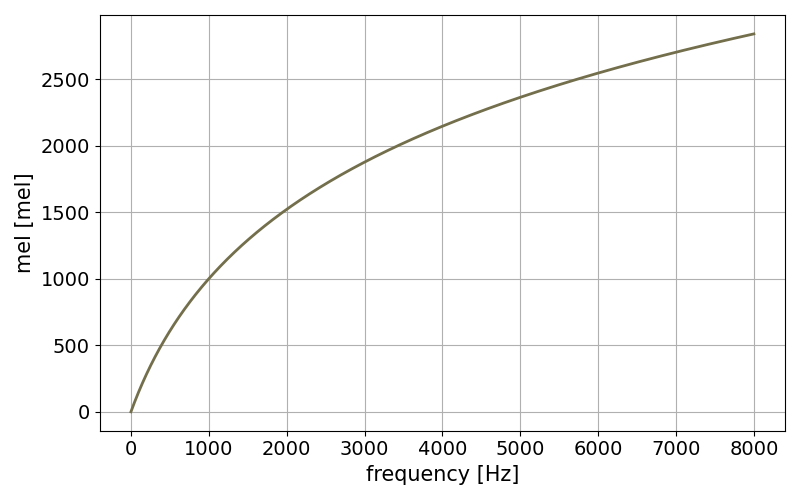
\includegraphics[width=0.40\textwidth]{./3_signal/figs/signal_mfcc_mel_scale}
  \caption{Mel scale as function of the frequency in a range of [0, \SI{8}{\kilo\hertz}].}
  \label{fig:signal_mfcc_mel_scale}
\end{figure}
\FloatBarrier
\noindent
The Mel and frequency window functions or equidistant Mel filter bands are shown in \rfig{filter_bands}.
\begin{figure}[!ht]
  \centering
  \subfigure[mel space]{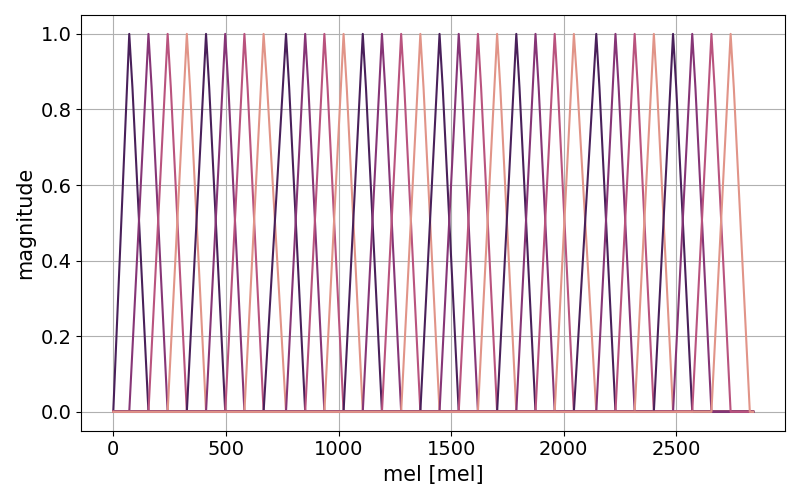
\includegraphics[width=0.40\textwidth]{./3_signal/figs/signal_mfcc_weights_mel}}
  \quad
  \subfigure[frequency space]{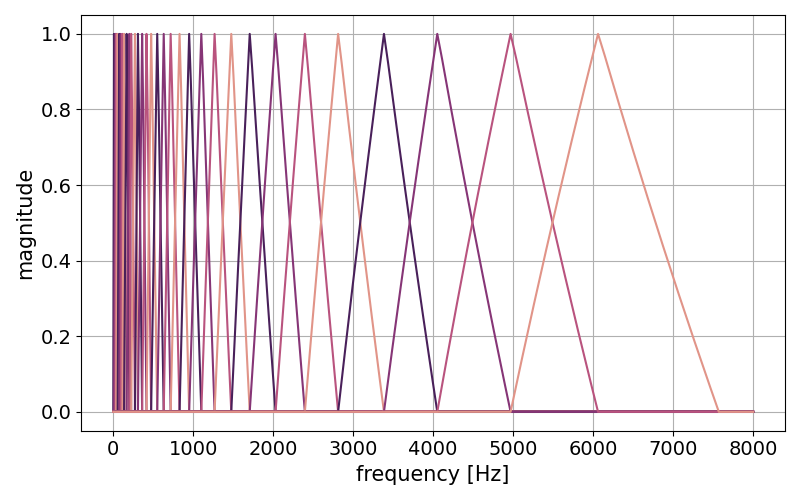
\includegraphics[width=0.40\textwidth]{./3_signal/figs/signal_mfcc_weights_f}}
  \caption{Equidistant Mel filter bands with a total number of 32 bands.}
  \label{fig:filter_bands}
\end{figure}
\FloatBarrier
\noindent
Note that the maximal frequency of the filter bands is $\SI{8}{\kilo\hertz}$, which is the half of the sampling frequency $f_s = \SI{16}{\kilo\hertz}$
The creation of those filter bands is not described mathematically, because the graphical showcase is much more intuitive and easier to understand.
For further calculations, those filter bands are notated in a weight matrix called $W_m \in \R^{B \times K}$, where $B$ are the amount of used filter bands as rows in the matrix and $K$ the amount of frequency bins of the DFT transformed input signal as columns.

% dct
The DCT is very similar to the Fourier transform and projects the input signal to a set of orthogonal basis functions, however the transformed signal is merely real valued instead of complex valued.
Different types of DCT formulations exist, but most commonly the \enquote{type 2} DCT is used and can be calculated as:
% dct
\begin{equation}\label{eq:signal_mfcc_dct}
  \hat{x}[c] = \sum_{n=0}^{N-1} x[n] \cos{\left[ \frac{\pi}{N} \left( n + \frac{1}{2} \right) c \right]}
\end{equation}
where $c$ is the DCT coefficient index and $n$ the sample index of a signal vector $\bm{x} \in \R^N$ with total length of $N$.
This can be conveniently written in matrix notation with a total number of $C$ DCT coefficients:
% dct matrix
\begin{equation}\label{eq:signal_mfcc_dct_matrix}
  \hat{\bm{x}} = \mathcal{D} \bm{x} \quad \mathrm{with} \quad \mathcal{D}[c, n] = \cos{\left[ \frac{\pi}{N} \left( n + \frac{1}{2} \right) c  \right]}, 
  \quad c, n = (0, 1, \dots, N - 1), (0, 1, \dots, C - 1) 
\end{equation}
with $\mathcal{D} \in \R^{C \times N}$ as DCT matrix and input signal $\bm{x} \in \R^N$ which gives the transformed signal $\hat{\bm{x}} \in \R^C$
The DCT basis functions illustrated in a matrix in two different color schemes are shown in \rfig{signal_mfcc_dct}.
\begin{figure}[!ht]
  \centering
  \subfigure[DCT with continuous color scheme]{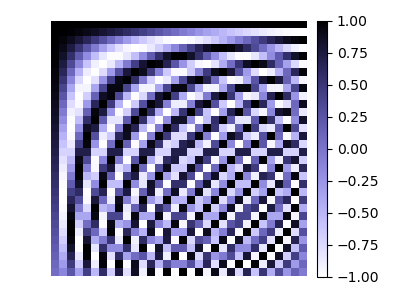
\includegraphics[width=0.35\textwidth]{./3_signal/figs/signal_mfcc_dct}}
  \qquad
  \subfigure[DCT with diverging color scheme]{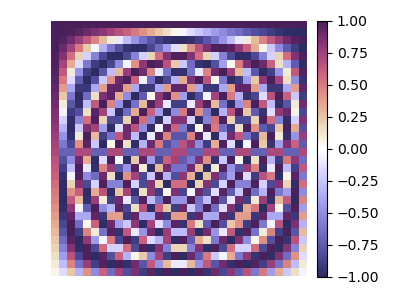
\includegraphics[width=0.35\textwidth]{./3_signal/figs/signal_mfcc_dct-div}}
  \caption{DCT matrix with 32 basis functions illustrated with a continuous and a diverging color scheme. The rows are the cepstral coefficients and the columns the length of the signal for transformation.}
  \label{fig:signal_mfcc_dct}
\end{figure}
\FloatBarrier
\noindent
The MFCCs $U \in \R^{C \times M}$ are calculated from the power spectrum of the STFT $P \in \R^{K \times M}$ computed in \req{signal_spec_spec}, the filter band weights collected in the matrix $W_m \in \R^{B \times K}$ and the DCT transformation matrix $\mathcal{D} \in \R^{C \times B}$ as following:
\begin{equation}\label{eq:signal_mfcc_mfcc}
  U = \mathcal{D} \log{ \left( W_m   P \right) }.
\end{equation}
Note that the rows of $U$ represent the cepstral coefficients and the columns the frames (shifts of the analytical window by the hop size).
The parameters for the computations of MFCCs are therefore the amount of filter bands $B$ and the amount of cepstral coefficients $C$.

Another important aspect is the visualization of MFCC features.
MFCCs computed as shown above, are not well intended for visualizations, because their individual coefficients value space differs strongly from each other.
For example the first coefficient equals a summation of all filter bands of the spectrogram and is therefore some kind of energy measure, while the other coefficients are different weighted sum combinations of the filter bands.
Further the most of the signal energy is located in the lower frequency bands, which impacts the value space of the coefficients with strongly weighted low frequency bands.
The differences in the value space leads to a problem in the visualization with a linear color scheme, so that some coefficients changes cannot be shown appropriately.
A solution to this problem is to normalize the feature vectors over each frame dimension with the infinity norm as:
% frame-based normalization
\begin{equation}\label{eq:signal_mfcc_norm}
  U[c, m] \gets \frac{U[c, m] + \vert \underset{m \in \mathcal{M}}{\min} \bm{u}_c \vert}{\norm{\bm{u}_c + \vert \underset{m \in \mathcal{M}}{\min} \bm{u}_c \vert}_\infty} \quad \forall \, c, m = (0, 1, \dots, C - 1), (0, 1, \dots, M - 1)
\end{equation}
where $c$ is the individual MFCC coefficient, $m$ the frame (time) index and $\bm{u}_c \in \R^M$ the individual MFCC coefficient vector over all frames $M$.
This equation gives a value space between $[0, 1]$ for each feature vector $\bm{u}_c$.
This normalization technique is denoted as frame-based normalization and it is an important evaluation subject in the following sections.

A visualization of MFCC features with 32 filter bands and 32 cepstral coefficients with frame-based normalization of each coefficient is shown in \rfig{signal_mfcc_showcase_mfcc32}.
\begin{figure}[!ht]
  \centering
    \subfigure[left]{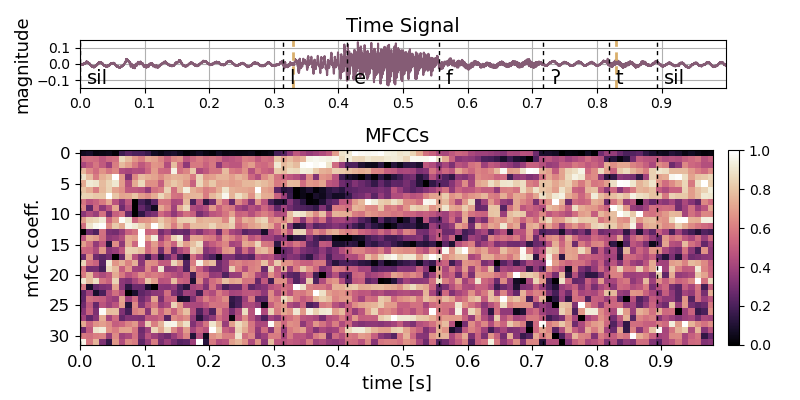
\includegraphics[width=0.45\textwidth]{./3_signal/figs/signal_mfcc_showcase_mfcc32_left0}}
    \subfigure[right]{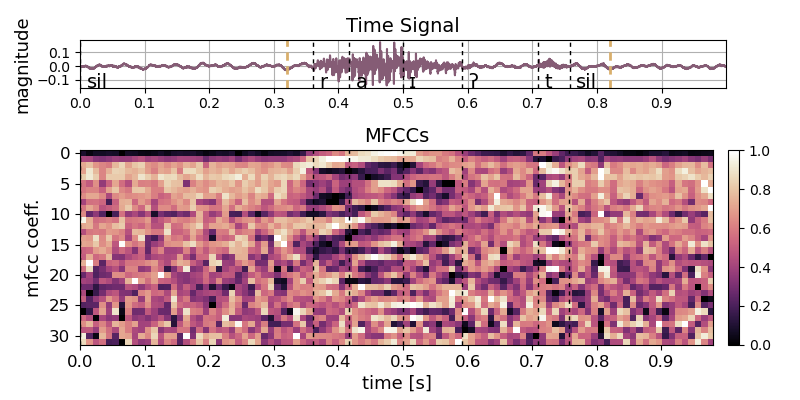
\includegraphics[width=0.45\textwidth]{./3_signal/figs/signal_mfcc_showcase_mfcc32_right0}}
    \subfigure[up]{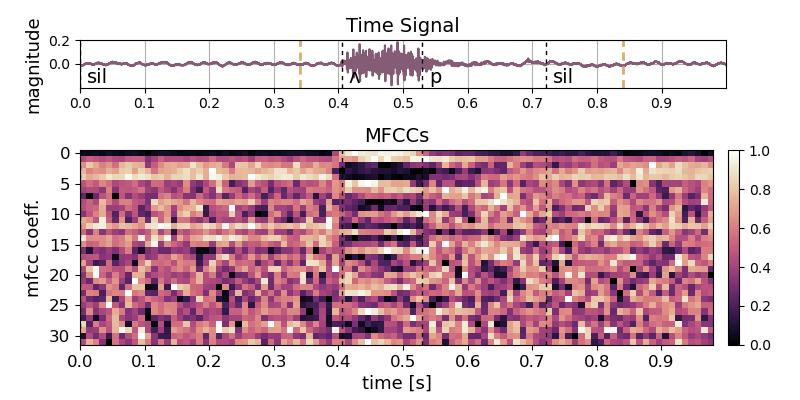
\includegraphics[width=0.45\textwidth]{./3_signal/figs/signal_mfcc_showcase_mfcc32_up0}}
    \subfigure[down]{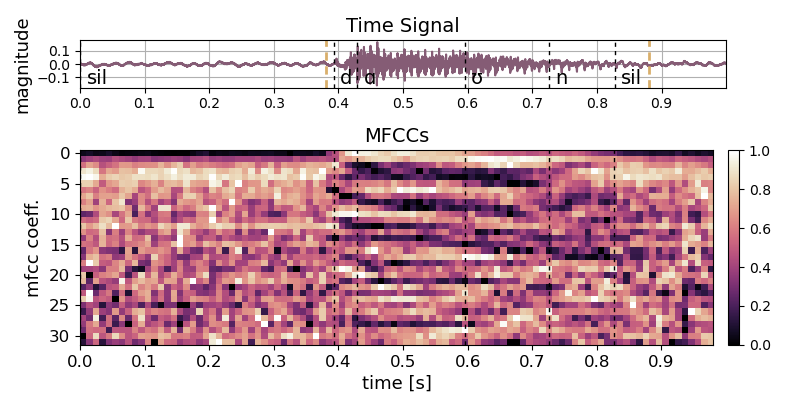
\includegraphics[width=0.45\textwidth]{./3_signal/figs/signal_mfcc_showcase_mfcc32_down0}}
    \subfigure[go]{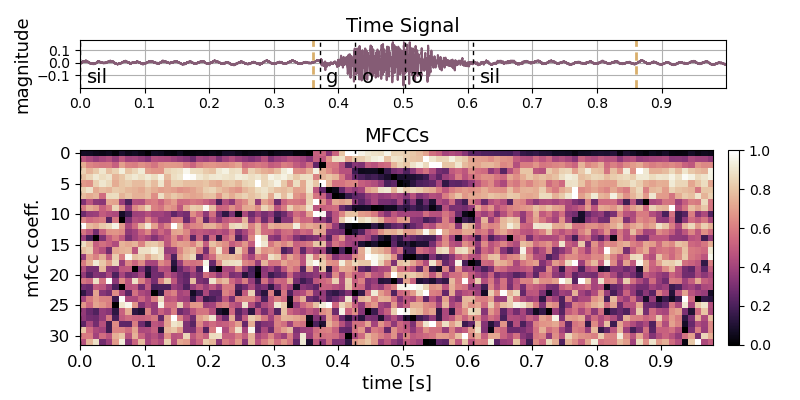
\includegraphics[width=0.45\textwidth]{./3_signal/figs/signal_mfcc_showcase_mfcc32_go0}}
  \caption{MFCC with 32 filter bands and 32 cepstral coefficients visualized with frame-based normalization.}
  \label{fig:signal_mfcc_showcase_mfcc32}
\end{figure}
\FloatBarrier
\noindent
The frame-based normalization is an interesting aspect to improve the visualization of the MFCC features, however it can be critical. 
A normalization that operates only in one dimension changes important structures within the feature space and it cannot be answered yet if this is a problem for neural networks or degrades the classification performance.
One more research question arises here: Is it possible to use frame based normalized MFCC features as inputs to neural networks and what are the results to the accuracy and training of the models.


% --
% enhancement

\subsection{MFCC Feature Usage and Enhancement}\label{sec:signal_mfcc_enhancement}
After the MFCCs are computed with the choice of filter bands $B$ and cepstral coefficients $C$, they can already be used as input features for neural networks.
The question arises, whether feature enhancement can improve the performance in classification.
The best practice, applied in many papers, is to use $B=32$, $C=12$, compute derivatives of those 12 MFCC coefficients named as deltas (first derivative regarding the frame dimension) and double deltas (second derivative) and add energy vectors of the 12 coefficients and each one of the deltas.
The deltas are simply computed as frame difference of the MFCCs with:
\begin{equation}\label{eq:signal_mfcc_delta}
  \Delta u_c[m] = \frac{u_c[m - 1] + u_c[m + 1]}{2}
\end{equation}
where $\bm{u}_c \in \R^M$ is the c-th MFCC coefficient vector and $m$ the frame index.
Note that the computation of the deltas at the edges $m=0$ and $m=M$ is not possible and the same value is obtained from the neighbor at this specific locations.
The second derivative of MFCC features, known as double deltas, are the frame differences of the deltas and in the same way computed as in \req{signal_mfcc_delta}.
Another enhancement is the computation of an energy feature vector of the MFCCs with:
\begin{equation}
  e[m] = \bm{u}[m]^T \bm{u}[m] 
\end{equation}
where $\bm{u}[m] \in \R^C$ is the MFCC feature vector of frame $m$.
The same energy computation may also be applied to the deltas and double deltas each.
The MFCCs, their deltas, double deltas and energy vectors can simply be stacked at top of each other and used as enhanced feature inputs to neural networks.
In this thesis the feature vectors are stacked as following:
\begin{enumerate}
    \item 12 MFCCs
    \item 1 Energy feature of the 12 MFCCs
    \item 12 Deltas
    \item 1 Energy feature of the 12 Deltas
    \item 12 Double Deltas
    \item 1 Energy feature of the 12 Double Deltas
\end{enumerate}
which sums up to a 39-dimensional feature vector, very commonly used in the literature.
Many papers do not explicitly explain how the 39 MFCCs are calculated in detail, in most cases however this constellation is applied.
The computation of 39 MFCCs are shown in \rfig{signal_mfcc_showcase_mfcc39}
\begin{figure}[!ht]
  \centering
    \subfigure[left]{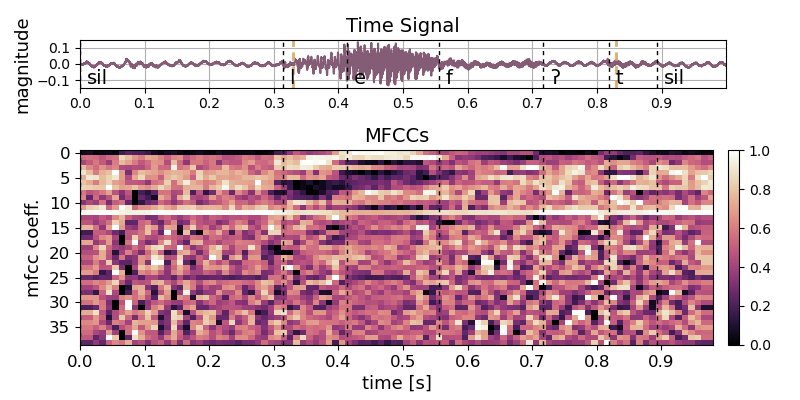
\includegraphics[width=0.45\textwidth]{./3_signal/figs/signal_mfcc_showcase_mfcc39_left0}}
    \subfigure[right]{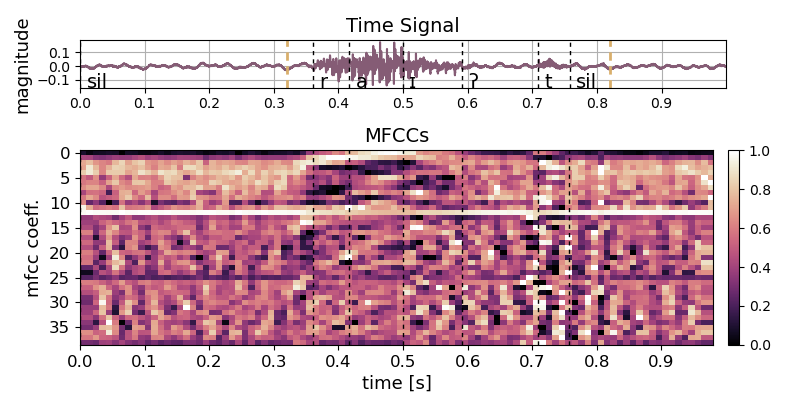
\includegraphics[width=0.45\textwidth]{./3_signal/figs/signal_mfcc_showcase_mfcc39_right0}}
    \subfigure[up]{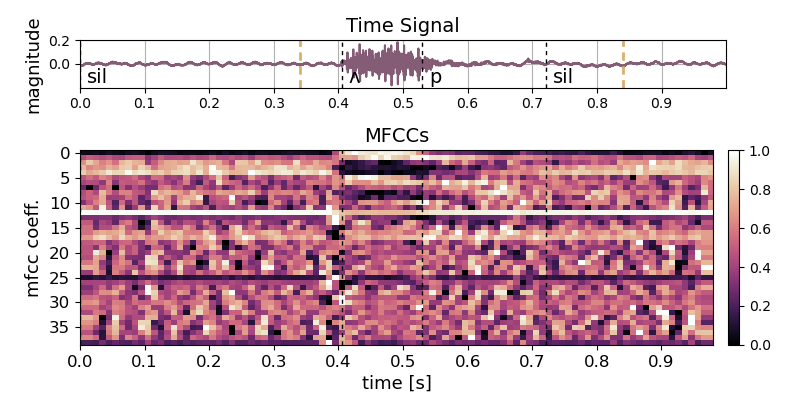
\includegraphics[width=0.45\textwidth]{./3_signal/figs/signal_mfcc_showcase_mfcc39_up0}}
    \subfigure[down]{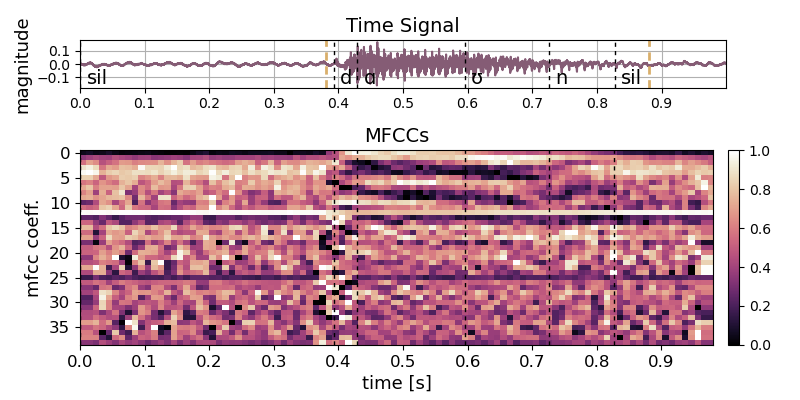
\includegraphics[width=0.45\textwidth]{./3_signal/figs/signal_mfcc_showcase_mfcc39_down0}}
    \subfigure[go]{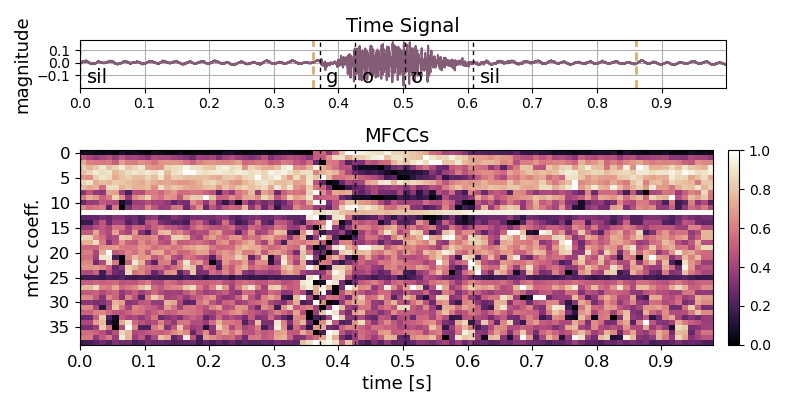
\includegraphics[width=0.45\textwidth]{./3_signal/figs/signal_mfcc_showcase_mfcc39_go0}}
  \caption{MFCC with 32 filter bands and 12 cepstral coefficients, deltas, double deltas and energy vector visualized with frame-based normalization.}
  \label{fig:signal_mfcc_showcase_mfcc39}
\end{figure}
\FloatBarrier
\noindent


% --
% energy consumption

\subsection{Computational Complexity}
The computational complexity is evaluated on the total amount of operations needed for a specific computation task, such as the feature extraction of MFCCs.
The energy consumption is related to the computational complexity, but it is much harder to define and depends on many parameters and actual hardware implementations, which is especially important for handheld devices.
The count of operations is sufficient for this thesis and provides a comparison to the benchmark models mentioned in \rsec{prev_kws_benchmark}.
The computational complexity for the extraction of MFCC features is the amount of operations needed to process a \SI{1}{\second} time signal sampled with $f_s = \SI{16}{\kilo\hertz}$.
All MFCC specific extraction details are collected in \rtab{signal_mfcc_extraction_params}.
\begin{table}[ht!]
\small
\begin{center}
\caption{Parameters for determining the computational complexity of the MFCC feature extraction process.}
\begin{tabular}{ M{7cm}  M{2.5cm} M{2.5cm}}
\toprule
\textbf{Parameter} & \textbf{Value} & \textbf{Sample Length} \\
\midrule
Length of a signal $n$ & \SI{1}{\second} & 16000 \\
Analytic window size $N$ & \SI{25}{\milli\second} & 400 \\
Hop size $h$ & \SI{10}{\milli\second} & 160\\
\midrule
Fourier coefficients $K$ & 400  & - \\
Number of filter bands $B$ & 32 & -\\
Number of cepstral coefficients $C$ & 12 & -\\
\bottomrule
\label{tab:signal_mfcc_extraction_params}
\end{tabular}
\end{center}
\vspace{-4mm}
\end{table}
\FloatBarrier
\noindent
The amount of operations are the total number of additions and multiplications necessary to fulfill the process.
The major components of the MFCC are, as described in \rsec{signal_mfcc_pipeline} and summarized in \req{signal_mfcc_mfcc}, the transformation to the STFT, the weighting with the filter bands and the DCT transform.
The most costly component is of course the STFT, which again is composed of Discrete Fourier Transforms (DFT).
Note that the DFT uses complex multiplications and additions.
One complex multiplication equals to 4 real multiplication and 2 additions, so one complex multiplication consists of 6 operations.
For one complex addition, two real additions are necessary and equals therefore to 2 operations.
A general matrix multiplication with a vector $y = A \bm{x}$, where $A \in \R^{m \times n}$ and $\bm{x} \in \R^n$ is composed of $m \cdot n$ multiplications and $m \cdot (n - 1)$ additions, where for simplicity the amount of additions is also assumed to be $m \cdot n$.

The amount of operations, denoted as $\mathcal{T(.)}$, for a trivial DFT transform with operator $\mathcal{F} \in \C^{K \times N}$ and $K$ Fourier coefficients on a windowed signal $\bm{x} \in \R^N$ with a total sample number of $N$ is:
\begin{equation}
  \mathcal{T}(\mathcal{F} \bm{x}) = 6 (N K) + 2 (N K)
\end{equation}
and give for $N = K = 400$ the amount of operations $\mathcal{T}(\mathcal{F} \bm{x}) = \SI{1.28}{\mega\ops}$ for a single DFT.
This of course are too many operations for a real time system, luckily a more sophisticated Fourier transform can be applied with the Fast Fourier Transform (FFT) algorithm \cite{Brigham1967}, which gives a linear complexity and operations are calculated as:
\begin{equation}
  \mathcal{T}(\mathcal{F} \bm{x}) = 6 (\mathcal{O}(N \cdot \log_2 N)) + 2 (\mathcal{O}(N \cdot \log_2 N))
\end{equation}
with $N = K = 400$.
The FFT has therefore roughly $\mathcal{T}(\mathcal{F} \bm{x}) = \SI{27.7}{\kilo\ops}$ and is a huge improvement to the trivial method.
%Further the interesting part of a DFT or FFT is only the half-band, because of the mirroring effect, which likewise may decrease the operations by half, so let the calculations be continued with Fourier coefficients of $K = 201$ of a half band and roughly $\SI{10}{\kilo\ops}$ per FFT.
The DFT is computed $M$ times, where $M$ is the total number frames calculated in \req{signal_spec_hop}, which gives $M = 98$ frames with the evaluated parameters.
So for the whole STFT the total number of frames $M$ is multiplied with the number of operations of each DFT, which give approximately $\mathcal{T}(\tilde{X}) = \SI{2.71}{\mega\ops}$.
Note that only the half-band of each individual FFT can be used, because of the mirroring effect at $\frac{f_s}{2} = \SI{8}{\kilo\hertz}$.
The Fourier coefficients are therefore reduced to $K = 201$.

The computation of the power spectrum and the log scaling are disregarded, so that two matrix multiplications remain:
$W_m P$ is a matrix multiplication of $\R^{B \times K}$ and $\R^{K \times M}$, which has $B K M$ real multiplications and approximately $B K M$ real additions, which give about $2 B K M = 2 \cdot 32 \cdot 201 \cdot 98 =  \SI{1.26}{\mega\ops}$.
The resulting band weighted power spectrum $\R^{B \times M}$ is further multiplied with the DCT operator, representing a matrix of $\R^{C \times B}$, that gives $2 C B M = 2 \cdot 12 \cdot 32 \cdot 98 = \SI{75}{\kilo\ops}$.
Altogether the matrix multiplications are approximately $\SI{1.26}{\mega\ops} + \SI{75}{\kilo\ops} = \SI{1.34}{\mega\ops}$.

The summary of the estimated operations are listed in \rtab{signal_mfcc_operations}.
% --
% mfcc operations
\begin{table}[ht!]
\begin{center}
\caption{Approximated number operations needed to transform a \SI{1}{s} time signal to MFCCs with parameters listed in \rtab{signal_mfcc_extraction_params}.}
\begin{tabular}{ M{6cm}  M{4cm}}
\toprule
\textbf{Process} & \textbf{Approximated Number of Operations} \\
\midrule
Power spectrum & \SI{2.71}{\mega\ops}\\
Weighting with equidistant Mel bands & \SI{1.26}{\mega\ops}\\
DCT transform of the weighted power spectrum & \SI{75}{\kilo\ops}\\
\midrule
\textbf{Sum} & \SI{4.05}{\mega\ops}\\
\bottomrule
\label{tab:signal_mfcc_operations}
\end{tabular}
\end{center}
\vspace{-4mm}
\end{table}
\FloatBarrier
\noindent


% --
% critism

\subsection{Criticism}
\thesisStateNew
MFCC are widely used for speech recognition tasks and perform very well, however the processing pipeline of MFCC has some disadvantages.
One disadvantage is, as already mentioned, that MFCCs are not intended for visualization, because of their broad value space of individual MFCC coefficients.
Another disadvantage is, that MFCC are not directly invertible to raw audio samples, because of the computation of the spectrogram.
Inversion techniques for MFCCs exist, such as described in \cite{Boucheron2008}, but it is still a rough approximation.
The inversion of MFCC would have been very interesting, when applied to generative neural networks, such as Generative Adversarial Neural Networks (GAN).